\documentclass[11pt,a4paper]{article}
\usepackage[T1]{fontenc}
\usepackage[utf8]{inputenc}
\usepackage{lmodern,microtype}
\usepackage[margin=25mm]{geometry}
\usepackage{amsmath,amssymb,booktabs,tabularx,longtable,array,enumitem}
\usepackage{xcolor,tikz,xurl,hyperref}
\usetikzlibrary{arrows.meta,positioning}
\definecolor{inkblue}{RGB}{25,65,100}
\hypersetup{colorlinks=true,linkcolor=inkblue,citecolor=inkblue,urlcolor=inkblue,
  pdftitle={Reasoning Through Interfaces: Random Closure Responses for Hyperon},
  pdfauthor={Mettapedia Working Notes}}
\setlength{\parindent}{0pt}
\setlength{\parskip}{5pt}
\setlength{\emergencystretch}{3em}
\setlist{itemsep=2pt,topsep=4pt}
\newcommand{\code}[1]{\nolinkurl{#1}}
\newcommand{\Pow}{\mathcal P}
\newcommand{\Fix}{\operatorname{Fix}}
\newcommand{\Prob}{\mathbb P}
\newcolumntype{P}[1]{>{\raggedright\arraybackslash}p{#1}}
\newcolumntype{Y}{>{\raggedright\arraybackslash}X}

\title{Reasoning Through Interfaces\\[3pt]
  \large Random Closure Responses for Modular Hyperon Systems\\
  An executive overview}
\author{Mettapedia Working Notes}
\date{1 November 2026}

\begin{document}
\maketitle

\begin{abstract}
A reasoning component can expose how it responds to future inputs while
hiding the internal derivations that produce those responses. For finite
positive recursive programs, MeTTapedia now proves that such interfaces
compose exactly, including feedback between components. A classical
commonality transform then turns the combination of independently uncertain
components into multiplication of prepared numerical rows. This joins
modular reasoning, explicit treatment of shared evidence, and local belief
updates in one mathematical account. The immediate opportunity is an exact
probability service for suitable ProbMeTTa and WM-PLN models; further uses
include chainers, compiler regions, distributed knowledge stores, and agent
memory. The Lean results and tested prototype exist. The ecosystem adapters
described here are proposed next work.
\end{abstract}

\section{A component can retain its response to future inputs}

Consider a large knowledge base divided into reasoning components: a diagnostic
module, a pathway model, a specialist's local rule set, or a region of a graph.
Most of each component's atoms are private. Other components interact with it
through a small set of named interface atoms $B$.

For fixed local random choices, let
\[
 C:\Pow(B)\longrightarrow\Pow(B)
\]
send an input set $S$ to the interface facts available after the component's
positive rules have reached their least closure. The response includes the
input facts. It is extensive, monotone and idempotent:
\[
 S\subseteq C(S),\qquad
 S\subseteq T\Rightarrow C(S)\subseteq C(T),\qquad C(C(S))=C(S).
\]
Private atoms may participate in multi-step and recursive derivations.
The interface retains their consequences for every possible seed.

This answers a practical memory question: \emph{what does another component
need to retain to cooperate with this one?} Within the declared observations,
its response operator suffices. The distinction matters even in the smallest
example. A component with rule $a\Rightarrow b$ and an empty component both
return nothing on the empty seed. Once $a$ arrives, their responses differ.
A snapshot of today's answer loses that distinction; the response profile
retains it.

\begin{figure}[ht]
\centering
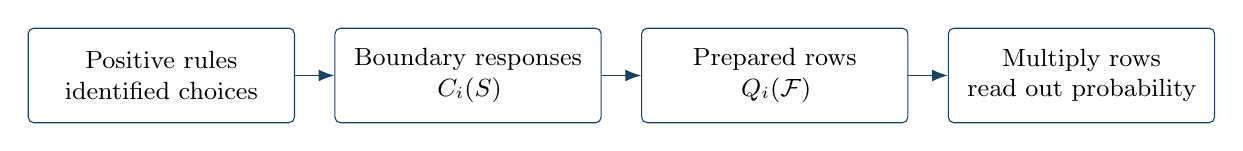
\begin{tikzpicture}[
  box/.style={draw=inkblue,rounded corners=2pt,align=center,
    text width=31mm,minimum height=12mm,inner sep=4pt,font=\small},
  >={Latex[length=2mm]},node distance=5mm]
  \node[box] (rules) {Positive rules\\identified choices};
  \node[box,right=of rules] (responses) {Boundary responses\\$C_i(S)$};
  \node[box,right=of responses] (rows) {Prepared rows\\$Q_i(\mathcal F)$};
  \node[box,right=of rows] (answer) {Multiply rows\\read out probability};
  \draw[->,inkblue] (rules) -- (responses);
  \draw[->,inkblue] (responses) -- (rows);
  \draw[->,inkblue] (rows) -- (answer);
\end{tikzpicture}
\caption{The representation separates local logical behavior from its current
probability weights. Reweighting uses retained local response data.}
\end{figure}

The opportunity is especially strong when internal reasoning is substantial,
the interface is small, and the rules stay fixed while evidence or priors
change repeatedly. A large internal implementation can then have a much
smaller externally sufficient description. This is an observation-relative
statement: it does not preserve every internal fact, derivation, trace,
effect, or future query someone might later request.

\section{Why independently built components can cooperate}

\subsection{Feedback is handled by a common fixed point}

For an operator $C$, write $\Fix(C)=\{T:C(T)=T\}$. If two components share
only their declared interface, the response of their combined rules is the
least closure above both responses, written $C\vee D$. Its defining law is
\[
 \Fix(C\vee D)=\Fix(C)\cap\Fix(D).
 \tag{1}
\]
An interface state is settled exactly when neither component can add anything.
The Lean development connects this algebraic construction to finite derivations
from the actual union of the components' rules and base facts.

For example, one component may infer $c$ from $b$, while another infers $b$
from $a$. Running the first component once and then the second on seed $a$
misses $c$. The joined closure includes both consequences. Consequently the
interface law supports cyclic communication; it does not require a one-way
pipeline of components.

The hypotheses identify real boundaries. All rule reads and conclusions must
belong to a component's scope, and private scopes must be disjoint outside the
interface. A further proved law admits shared input atoms when all components
agree on their values and no rule can redefine them. Hidden cross-component
references do not satisfy this contract.

\subsection{Uncertainty can be moved into compositional coordinates}

Random local choices select different response operators. For a finite family
of candidate interface states $\mathcal F$, define
\[
 Q_C(\mathcal F)
   =\Prob\bigl(\forall T\in\mathcal F,\ C(T)=T\bigr).
 \tag{2}
\]
The probability is over the model's identified random choices.
This is a \emph{joint} observation: every state in the family must remain
closed under the same realized component. For independently chosen components,
(1) gives
\[
 Q_{C\vee D}(\mathcal F)=Q_C(\mathcal F)Q_D(\mathcal F).
 \tag{3}
\]
Thus logical feedback becomes intersection of fixed-point families, and
independent uncertainty becomes pointwise multiplication. The latter is the
classical commonality law for conjunctive combination on lattices
\cite{denoeux}. Probabilistic argumentation already connects logical inference
and belief-function representations \cite{haenni}. The contribution here is
the checked composition from source rules through hidden interfaces to query
probability, together with a concrete update prototype. Priority for a new
general inference method is not claimed.

Different component names or source labels do not establish stochastic
independence. If components use a common random input $h$, the combination is
instead computed conditionally:
\[
 Q(\mathcal F)=\sum_h w(h)\prod_i Q_i^h(\mathcal F).
 \tag{4}
\]
The shared choice is weighted once. The formal source laws make both
factorization and consistent treatment of shared inputs explicit.

\subsection{A two-component example explains the dependence boundary}

Let the interface be $\{a,b,c\}$. The first component can derive $b$ from $a$
when event $x$ holds; the second can derive $c$ from $b$ when event $y$ holds.
From seed $\{a\}$, the event of deriving $c$ is $x\land y$. If $x$ and $y$ are
independent fair events, the answer is $1/4$. If both stages depend on the
\emph{same} fair observation, the answer is $1/2$.

This is directly relevant to agents that repeat or reuse one another's
evidence. Two supporting steps need not represent two independent events.
At the logical level, $C\vee C=C$; this does not license $Q^2=Q$ for independent
draws from a distribution of closures. A replayed message about an identified
component is a revision or duplicate to handle by identity, not a new
independent component to multiply into the belief.

\section{Recovering answers and updating beliefs}

The commonality rows retain enough information to answer membership queries.
For seed $S$ and queried interface atom $q$, let
\[
 \mathcal A_{S,q}=\{T\subseteq B:S\subseteq T,\ q\notin T\}.
\]
The statement $q\notin C(S)$ is equivalent to the existence of a closed
$T\in\mathcal A_{S,q}$. Finite inclusion--exclusion therefore gives
\[
 \Prob(q\in C(S))=
 \sum_{\mathcal F\subseteq\mathcal A_{S,q}}
       (-1)^{|\mathcal F|}Q_C(\mathcal F).
 \tag{5}
\]
For the example above, $\mathcal A_{\{a\},c}=\{\{a\},\{a,b\}\}$. Its answer is
\[
 1-Q_C(\{\{a\}\})-Q_C(\{\{a,b\}\})
      +Q_C(\{\{a\},\{a,b\}\}).
\]
The last, joint term is essential. Keeping only individual closed-state
probabilities would lose the dependence required for exact extraction.

A prepared query bank can merge families with the same intersection closure
and add their signed coefficients. Lean proves this reduction preserves the
answer. The prototype retains the required rows, local choice-to-response
profiles, and a balanced tree of component products. Updating local weights
or evidence replaces the affected rows and recomputes ancestor products.
No division by an old contribution is needed, so zero weights remain valid.
Current $Q$ values alone would not be enough to perform arbitrary reweighting;
the retained response data or another justified row updater is necessary.

For $N$ components, $K$ retained rows, at most $k$ private random choices per
component, and $d$ updated components, the intended arithmetic-operation cost is
\[
 O\bigl(dK2^k+dK\log N+\text{query extraction}\bigr).
\]
Initial response construction, arithmetic bit cost, and exact fallback add
cost. Enumerating shared choices adds a factor of $2^h$ for $h$ shared Boolean
inputs. Both local choice count and interface width matter: the observation
families in (5) can grow very quickly, even after merging.
A module boundary therefore has a computational meaning: it identifies the
information needed to keep other components' answers correct after local change.

Evidence is kept unnormalized until the final readout. Zero evidence mass
produces no conditional answer; an ordinary zero probability remains a valid
answer. The prototype uses outward-rounded intervals and rational fallback
when cancellation prevents the required enclosure. Its numerical implementation
is separately tested, rather than extracted from the Lean proofs.

The cheap update path assumes the same admitted rules, interface and choice
schema. New rules, new event identities or a different boundary require
rebuilding the relevant responses and checking the contract again. Observing
a combined conclusion can also correlate components: the factorization in
(3) must still hold, or be recovered through an explicit separator such as (4).

\section{Where this can help Hyperon}

The following are proposed integration targets. The existing formal and
software footholds are identified in the source inventory below; a foothold
is not a completed adapter.

\begingroup\small
\renewcommand{\arraystretch}{1.12}
\begin{longtable}{@{}P{.18\textwidth}P{.37\textwidth}P{.37\textwidth}@{}}
\toprule
Destination & Useful role & Necessary integration work \\
\midrule
\endfirsthead
\toprule Destination & Useful role & Necessary integration work \\
\midrule
\endhead
\bottomrule
\endfoot
ProbMeTTa and WM-PLN &
Exact recurring queries over modular positive models; update local priors and
evidence while retaining the source-probability correspondence. &
Build finite response tables and an executable readout for the normalized
source and query bank. Supply a joint model beyond scalar truth values.
\\[5pt]
PeTTaChainer and mm2-chainer &
Reuse finite ground positive subprograms for repeated support and diagnostic
queries, keeping shared base events separate from the number of derivations. &
Admit the region and observer; preserve requested proofs separately.
Entailment probability certifies neither a proof object nor a budgeted
search's success rate.
\\[5pt]
CeTTa and Prime; compiler lowering &
Lower an admitted probability observation to this service. The same contract
could guide future Cesta/Sexos lowering. &
Prove the language/profile bridge. Preserve ordered, bag and effect observations
where required. Prime still needs a checker-accepted certificate.
\\[5pt]
GSLT and MeTTaIL &
Give suitable module interfaces a probabilistic meaning; guide module
discovery toward small coupling boundaries and explicit preserved observations. &
Extract positive ground components and certify scope. Consumption, negation
and arbitrary rewrites need other semantics; automatic partition discovery
remains open.
\\[5pt]
MORK and PathMap &
Store shared response profiles and indexed component updates alongside the
existing storage and execution substrate \cite{mork,pathmap}. &
Bind rows to component identities and revisions; implement numeric reduction.
A trie join alone does not implement the probability product.
\\[5pt]
AtomSpace, DAS and federated reasoning &
Expose reasoning-region summaries to DAS \cite{das} or other federated query
services, reducing what a shard must exchange for the declared queries. &
Maintain model revisions, coverage, shared causes and event ownership.
Deduplicate deliveries; prove the distributed snapshot and transport contract.
\\[5pt]
G\"odelClaw and collaborating agents &
Give specialists small logical response models at their workspace interface,
counting shared observations once across collaborating agents. &
Keep context epochs and source identities. Restrict the service to pure
reasoning; participation and executable tool authority remain external.
\\[5pt]
Memory, retrieval and attention &
Retain distinctions needed for declared future inputs; supply model-relative
probabilities to retrieval and inference-control policies. &
Connect memory and retrieval contracts. Minimal memory, privacy and optimal
attention need additional results; changing the query family requires renewed
sufficiency.
\\[5pt]
Scientific and graph models &
Update finite pathway, diagnostic or uncertain-reachability models as evidence
changes, using small interfaces between regions. &
Justify the world model and dependence. Inhibition, temporal resampling and
causal interventions need additional encoding; exact arithmetic does not
validate the model.
\\
\end{longtable}
\endgroup

Two distinctions are particularly useful across these applications.
\emph{Semantic hiding} says which internal details a declared observer can
ignore; it is not an information-security guarantee. \emph{Logical closure}
is idempotent, but probabilistic message processing still needs source identity,
versioning, and justified independence. These are reasons to make the interface
explicit before distributing or caching it.

\section{A practical first integration}

The nearest useful deployment path is a narrow ProbMeTTa/WM-PLN query service.
Its first artifact should be an executable finite response-table builder and
rational evaluator connected to the existing Lean correspondence. This closes
the gap between the semantic construction and the tested numerical prototype.

A consumer-facing component record should identify its source rules, interface,
choice ownership, shared inputs, allowed queries and model revision. It should
carry enough retained local information to recompute rows after admissible
weight changes. Unsupported requests should be routed to an appropriate
existing engine; impossible evidence should retain its distinct no-answer
status. Exactness is relative to the supplied world model: a retrieved subset
of a knowledge base needs a coverage argument before its answers can stand for
the whole source region.

The first application can be a finite diagnostic or reachability model with
stable rules and recurring evidence updates. After that service has a source
and observation bridge, a chainer or runtime can reuse it within an admitted
region. For large local choice sets, the existing local BDD compiler is a
natural future way to obtain component rows without enumerating every local
world. The global commonality composition can remain the same.

This development order focuses on useful integration and small correctness
controls. The mathematical value is already present: internal reasoning,
shared uncertainty, and changing beliefs now have a common, explicit account
of what a component exposes and what composition preserves.

\section{What is established}

The qualified snapshot of 1 November 2026 contains two new Lean modules,
with 201 owned declarations audited for admissions and foundational
dependencies. The proofs use only Lean's standard \code{propext},
\code{Classical.choice}, and \code{Quot.sound}; no custom axioms or admitted
proofs were introduced. The source-to-response laws, prepared extraction,
shared-input conditions and agreement with the existing probability semantics
are proved. Python and C++ execution remain separately tested implementations.

Controls cover feedback that needs more than one pass, self-loops without external support,
responses indistinguishable on the empty seed, shared versus independent
events, private-atom leakage, zero/one weights, and impossible evidence.
The numerical prototype exercised 180,000 updates and 360,000 answers across
the small-interface workloads, with the recorded numerical-width checks
passing. These observations support engineering feasibility. Comparative
performance and system-wide impact remain empirical questions.

The scope is finite positive reasoning with declared observations and a
justified probability model. Wider interfaces, many local choices, global
churn and cancellation can erase the advantage. Arbitrary MeTTa execution,
negation, proof-trace preservation, distributed consistency and runtime
authorization remain separate obligations.

\clearpage
\section{Measured behavior of the prototype}

The recorded experiment used positive recursive components with three interface
atoms, four private random choices and eight private atoms per component.
It included unary and multi-premise rules; templates could share preparation
under atom renaming. Activation probabilities scaled as $1/N$. Each run made
10,000 updates and queried two targets from one fixed interface seed: 80\% of
updates targeted probabilities, and 20\% targeted evidence within a fixed bank
of at most eight components. The timed models had no shared random inputs;
shared choices were covered by correctness controls.

All 18 commonality runs completed. The following wall-time ranges include
preparation and cover generator seeds 7, 19 and 43; they are single-stream
observations on a shared x86-64 workstation, not confidence intervals.

\begin{center}
\begin{tabular}{@{}rrr@{}}
\toprule
Components & One component updated & Four components updated \\
\midrule
256   & 2.11--2.16 s & 6.12--6.23 s \\
1,024 & 2.49--2.74 s & 7.66--8.20 s \\
4,096 & 3.09--3.62 s & 9.10--9.47 s \\
\bottomrule
\end{tabular}
\end{center}

All 360,000 answer enclosures met absolute width $10^{-12}$ and relative width
$10^{-10}$ for positive answers, without rational fallback in these runs.
The commonality implementation used 34-digit outward-rounded decimal arithmetic.

An \emph{exploratory} stronger comparator used
\href{https://proceedings.kr.org/2021/26/kr2021-0026-eiter-et-al.pdf}{ASPMC}'s
counting-safe TP unfolding and d4, with exhaustively tested private-rule unfolding and
specialization to the stream's fixed seed. A C++ evaluator cached the actual
compiled arithmetic DAG and updated affected ancestors, stopping at unchanged
values. Its ordinary floating-point answers were checked against the declared
accuracy tolerances. The 256-component, seed-7, one-component-update case gave:

\begin{center}
\begin{tabular}{@{}lrrr@{}}
\toprule
Method & Preparation & 10,000 updates & Total \\
\midrule
Commonality & 0.03 s & 2.10 s & 2.13 s \\
ASPMC/d4, cached ancestors & 7.99 s & 3.43 s & 11.42 s \\
ASPMC/d4, reassociated cache & 10.20 s & 3.18 s & 13.39 s \\
\bottomrule
\end{tabular}
\end{center}

Preparation includes source preprocessing, compilation and arithmetic
export/cache construction for the comparator; tool installation and
benchmark-input generation are excluded. The software was CPython 3.13.13,
ASPMC 1.1.1 and GCC 15.2.0. All 10,000 answers from both incremental variants
passed validation. Against the faster total, the measured advantage was
\textbf{5.37$\times$ overall}, but only \textbf{1.5--1.6$\times$ during updates}.
Much of the total advantage therefore comes from preparation.

The ablations clarify the mechanism and its limits. At 256 components, direct
closure-distribution convolution with the same local-update tree took 73.90 s,
versus 2.13 s for commonality. Under global churn, both local maintenance and
full recomputation took about 1.30 s (64 components, 200 updates). Interface
widths three, four and five required 13, 75 and 541 rows. In a two-component
rare-query control (answers around $10^{-100}$), commonality used rational
fallback on all 1,000 updates and took
0.108 s, versus 0.062 s for direct convolution.

\textbf{Qualification boundary.} This completed comparison is exploratory and
at 256 components. The strengthened 1,024-component compilation timed out
after 120 s; no 4,096-component escalation followed. Full cached native
evaluation at 256 also stopped after 112 updates, so it supplies no completed
10,000-update timing. Timeouts are not converted into speedup ratios.
The registered fourfold claim at 1,024 and 4,096 remains unqualified.

\clearpage
\appendix
\begingroup\small
\setlength{\parskip}{3pt}
\setlist[itemize]{itemsep=1pt,topsep=2pt}
\section{Source inventory and review anchors}

All Lean paths below are relative to \code{lean/mettapedia/Mettapedia/} in the
MeTTapedia repository \cite{mettapedia}. The two new sources are
\code{Logic/RandomClosure.lean} and
\code{Logic/BDD/ClosureResponseCounting.lean}. Their namespaces are respectively
\code{Mettapedia.Logic.RandomClosure} and
\code{Mettapedia.Logic.BDDCore.ClosureResponseCounting}.

\begingroup\small
\begin{tabularx}{\textwidth}{@{}P{.50\textwidth}Y@{}}
\toprule
Declaration & Review purpose \\
\midrule
\code{join_closed}, \code{combine_closure} & Fixed-point algebra and actual rule union. \\
\code{response_combineFamily_readonly} & Hiding with explicit immutable shared inputs. \\
\code{commonality_family} & Factorization over independent local choices. \\
\code{preparedExtract_correct} & Exact query extraction after merging equal intersection closures. \\
\code{conditioned_component_query_mass} & Shared choices weighted once around actual component execution. \\
\code{factored_queryProb} & Source partition and weight factorization connect to ProbLog probability. \\
\code{agrees_with_certified_count} & Agreement with the existing certified BDD route. \\
\code{sourceProbability_correct} & Positivity-checked source observation. \\
\code{conditionalResponse_none_iff} & Zero evidence mass gives no conditional answer. \\
\bottomrule
\end{tabularx}
\endgroup

Existing integration footholds include:
\begin{itemize}
\item \code{Logic/BDD/CertifiedProgramProbability.lean} and
  \code{Logic/BDD/ProbMeTTaEndToEnd.lean}: source and counting semantics.
\item \code{ProbabilityTheory/BayesianNetworks/SeparatorFactorization.lean}:
  the separator sum/product law reused by the shared-choice bridge.
\item \code{Evidence/SourceScopeProbabilityBoundary.lean}:
  provenance separation and stochastic independence are distinct.
\item \code{Machines/RecursiveInsertRegion.lean}: observer-qualified selection
  within an already admitted finite Horn region.
\item \code{GSLT/Logic/TaskRelativeMemory.lean} and
  \code{Algorithms/Retrieval/RetrievalContract.lean}: future-observation
  sufficiency and exact retrieval obligations.
\item \code{CognitiveArchitecture/GodelClaw/GlobalWorkspace.lean} and
  \code{CognitiveArchitecture/AttentionEconomy.lean}: existing context,
  specialist, effect and attention boundaries for proposed agent adapters.
\end{itemize}
The numerical prototype and comparison adapters are under
\code{lean/mettapedia/scripts/benchmarks/closure_response*}.
These source anchors identify the current mathematical footholds, not completed
runtime integrations.

\begin{thebibliography}{9}
\bibitem{denoeux}
T.~Den\oe ux and M.-H.~Masson.
\emph{Dempster--Shafer reasoning in large partially ordered sets:
Applications in Machine Learning}. BELIEF, 2010.
\url{https://bfasociety.org/Belief2010/html/papers/p70.pdf}.

\bibitem{haenni}
R.~Haenni and N.~Lehmann.
\emph{Probabilistic argumentation systems: A new perspective on the
Dempster--Shafer theory}. International Journal of Intelligent Systems
18(1):93--106, 2003. \url{https://doi.org/10.1002/int.10076}.

\bibitem{mork}
MORK project. \emph{MeTTa Optimal Reduction Kernel}.
\url{https://github.com/trueagi-io/MORK}.

\bibitem{pathmap}
PathMap project. \emph{PathMap documentation}.
\url{https://pathmap-rs.github.io/}.

\bibitem{das}
DAS project. \emph{Distributed Atom Space: conceptual documentation}.
\url{https://github.com/singnet/das/blob/master/docs/conceptual_documentation.md}.

\bibitem{mettapedia}
MeTTapedia project. \emph{Formal source library and working papers}.
Source snapshot reviewed 1 November 2026.
\url{https://github.com/zariuq/MeTTapedia}.
\end{thebibliography}
\endgroup
\end{document}
